
\documentclass[12pt,a4paper]{book}

%\documentclass[a4paper,12pt]{article}


\usepackage{verbatim}
\usepackage{cite}
%\usepackage[square]{natbib}
\usepackage{parskip}
%\usepackage{longtable}
\usepackage{listings}
\usepackage{graphicx}
\usepackage{float}
\usepackage{rotating}
\usepackage{appendix}
\usepackage{amsmath}
\usepackage{longtable}

\usepackage[Lenny]{fncychap}

\usepackage{color}
\definecolor{Grey}{rgb}{0.5,0.5,0.5} 






% Make margin of captions smaller
%\usepackage[margin=1cm]{caption}

%\usepackage{fancyhdr}
%\pagestyle{fancy}

% BNF Grammar stuff
\usepackage{syntax}
\newdimen\grammarindent
\grammarindent10em
%\renewcommand{\syntleft}{\normalfont\itshape}
%\renewcommand{\syntright}{}
\renewcommand{\sdsize}{%
\scriptsize%
}


% Listings stuff
\usepackage{xcolor}
\usepackage{caption}
\DeclareCaptionFormat{listing}{%
  \parbox{\textwidth}{\colorbox{Gray}{\parbox{\textwidth}{#1#2#3}}\vskip-4pt}}

\lstset{ %
basicstyle=\scriptsize,         % the size of the fonts that are used for the code
%basicstyle=\ttfamily,
%numbers=left,                   % where to put the line-numbers
%numberstyle=\scriptsize,        % the size of the fonts that are used for the line-numbers
%frame=trBL%single,                   % adds a frame around the code
frame=single,
framerule=1pt,
frameround=tttt,
%backgroundcolor=\color{red},
showstringspaces=false,
tabsize=2,                      % sets default tabsize to 2 spaces
captionpos=b,                   % sets the caption-position to bottom
breaklines=true,                % sets automatic line breaking
breakatwhitespace=false,        % sets if automatic breaks should only happen at whitespace
%title=\lstname,			% include title (file name)
xleftmargin=5pt,
xrightmargin=5pt,
%framextopmargin=45pt.
%framexbottommargin=45pt,
rulecolor=\color{Grey}
}

\newcommand{\inhas}[1]{\texttt{'#1'}}

% Disable section numbering
%\setcounter{secnumdepth}{-1} 


\begin{document}

\title{Just-In-Time compilation of\\Haskell with PyPy and GHC}
\author{Author:\\
Knut Halvor Skrede\\
\\
Supervisor:
\\
Dr. Magnus Lie Hetland}

%\pagestyle{}
\pagenumbering{roman}

\begin{titlepage}
\maketitle
\end{titlepage}


\chapter*{Abstract}

The abstract.

\clearpage

\chapter*{Preface}

\section*{Acknowledgements}

I would like to thank the following people;

\begin{itemize}

\item Carl Friedrich Bolz, for his help on both the technical parts
of the project, and on the formulation of this report.

\item My supervisor, Magnus Lie Hetland, for all his help.

\item Even Wiik Thomassen, for his help and hard work.

\item My friends and family for their support during these years of study.

\end{itemize}


\section*{Disclaimer}

This is a collaboration project. Two people are working on this
project at the same time; me, and Even Wiik Thomassen. Since I am working
on my master thesis and he is working on his specialization project, we 
write separate reports. We attempt to present our work in such a way that
it is clear who has done what. Some parts may however look similar,
especially the introduction and background parts, as they are based on 
some of the same papers.



\clearpage

\setcounter{tocdepth}{2}
\tableofcontents
%\clearpage
%\listoffigures
%\listoftables
%\clearpage
\clearpage

\pagestyle{plain}
\setcounter{page}{1}
\pagenumbering{arabic}


\chapter{Introduction}

This chapter discusses the motivation behind the project and 
presents a description of the project and of the work done. It 
is concluded by introducing the remaining chapters.

\section{Motivation and project description}

The project aims to investigate the feasibility of JIT (Just-in-time) 
compilation of a strongly-typed purely-functional language. Since
programs written in such a language can be heavily optimized at 
compile time, it is uncertain whether such programs can benefit from
JIT compilation. However, a JIT compiler has a lot more information to
work with than a static compiler. 

To test this, the techniques 
used by the PyPy (Python in Python) project are applied to the Haskell 
programming language. By implementing the back-end for a Haskell compiler 
in RPython (restricted Python), and using GHC (the Glasgow Haskell Compiler) 
as a front-end, a full Haskell JIT compiler can be implemented. An 
interpreter for a language very similar to the intermediate language used
by GHC was already implemented, and this is the base for this project.
Although it is already possible to have JIT compilation with GHC through
its LLVM back-end, the PyPy approach will interpret code at a much higher level.

We focus on implementing a serializer from Haskell to an intermediate
format using GHC, and a deserializer from that format to the interpreter. The 
interpreter is for a language similar to Core (the intermediate format used by GHC.)
By implementing some simple programs in Haskell, and running them through our 
compilation system, 
we hope to show that the methods of the PyPy project can be successfully applied 
to pure functional languages such as Haskell.

\section{Contributions}
The contributions of this thesis is a description of Haskell-Python (an
interpreter for Core' (a lambda-calculus inspired by Haskell)), and a system for
translating Haskell programs into Core'. In addition to this, the paper 
presents a description of the full compilation system in its current state,
and a plan for the future development of the system based on the 
successes and failures so far.

Following is a listing describing how the work in this project has been
partitioned.

The following work had already been done:
\begin{itemize}

\item The Haskell-Python\cite{haskellpython} interpreter was written.

\end{itemize}

These parts were the result of an earlier stage of the project:
\begin{itemize}

\item An investigation into the use of GHC as a front-end for the compiler.
This resulted in the JSCore intermediate language, but was unsuccessful
at creating JSCore files from the GHC Haskell libraries.

\item A parser for the JSCore language was implemented; however, this 
parser was only successful for a very small subset of the JSCore language.

\item A simple system for testing functionality was implemented.

\end{itemize}

For this project, the following has been done:
\begin{itemize}

\item Another attempt was given at the creation of JSCore for the GHC 
Haskell libraries, but was still unsuccessful. The reason for this being
bugs in GHC. Specifically, bugs in the code that dumps the External-Core
files.

\item Various Haskell values and functions have been implemented at a higher
level. Due to the fact that we could not successfully create intermediate
files for the Haskell
libraries we had to implement the functionality at a higher level, i.e. 
Python.

\item Based on the gained understanding of the Core language from the
previously mentioned work, the parser has been improved. The result of 
the improvements to the parser, with the implementation of the libraries,
has resulted in the successful execution of some less trivial programs,
such as a naive recursive implementation of fibonacci.

\end{itemize}

In addition to this, some work has been done in parallell by E.W.Thomassen,
most notably:
\begin{itemize}

\item Refactoring of the code written previously, in order to make it better 
match other PyPy projects.

\item Rewriting the Python code into RPython, such that it can be translated by
the PyPy toolchain.

\item He has also changed quite a bit of the functionality for the better,
and details of this work can be found in his report.

\end{itemize}

% Write about the use-cases of laguages like Haskell, and the benefits of 
% Jit compilation

% + Research blahblah... Just to see if it works well.

% Structure of the paper. TODO
\section{Structure of the paper}
In chapter \ref{chap:back} some background information is presented, including 
some terms and concepts. 
%
A description of the 
Haskell-Python interpreter is given in chapter \ref{chap:hs}.
%
Chapter \ref{chap:rewrite} goes into detail regarding the intermediate 
languages, and the mapping between them.
%
%In chapter \ref{chap:prims} the Haskell libraries and necessary primitives
%are discussed.
%
%Chapter \ref{chap:pipe} describes the entire pipeline of the compilation system 
%at a high level.
%
%Chapter \ref{chap:test} describes the test-system used.
%
Chapter \ref{chap:impl} contains a description of the compilation system.
%
In chapter \ref{chap:similar} a brief discussion of similar work is presented.
%
Chapter \ref{chap:bench} presents some preliminary benchmark results.
%
Everything is concluded in chapter \ref{chap:conc}, which discusses 
the results and future work.

%\clearpage

\section{Background}
\label{chap:back}

\subsection{Haskell}

% What is Haskell ?
Haskell is a lazy, pure functional language with non-strict semantics and static 
polymorphic typing. It provides user-defined algebraic datatypes, pattern-matching, 
list comprehensions, a system for modules, a system for monadic I/O, and a large 
standard library. In addition to beeing strongly typed, Haskell supports type
inference, which means type annotations are seldom required. We do not go into 
too much detail here, for a full description 
of Haskell, see "the Haskell 2010 language report"\cite{marlow2010haskell}. 
Or for a complete history of Haskell, see "A history of Haskell: being lazy 
with class"\cite{hudak2007history}.

Two specific features
of Haskell stand out: it is purely functional; this means that the functions 
can not have side-effects, or mutate data. For equal arguments, a function 
must provide equal results. The fact that Haskell is lazy refers to the techniques
used to evaluate a Haskell program, meaning that the arguments to a function are passed
unevaluated, and only evaluated when needed. Lazy semantics also means that impure 
non-functional language features are impossible, as the two cannot work in conjunction.
\cite{marlow2010haskell, marlow2012glasgow}

\subsection{PyPy}

% What is the PyPy project ?
PyPy is a project that shows the feasability of constructing a VM (Virtual Machine) 
for a dynamic  language in a dynamic language, specifically, Python. The PyPy 
environment aims to translate (i.e. compile) the VM into arbitrary targets. This 
means that an interpreter constructed in the PyPy environment will be able to 
run on any target supported by PyPy. Instead of writing multiple versions of 
the interpreter (one for C/Posix, JAVA, and one for CLI/.NET), it can be 
written in RPython, and translated to those back-ends. PyPy uses the 
"meta-programming" argument, if the VM can be written at a level of abstraction 
high enough, then it can be translated to any lower level platform. Implementing 
programming languages using a direct encoding approach is a complex task, and it 
usually results in an implementation that is specifically designed for a target platform. 
In effect this means that the implementation is not generic, and it is difficult to 
reuse the code for anything other than it's specific purpose. In contrast, 
PyPy's approach puts weight on portability and reusability\cite{pypy}. Although the
PyPy project puts most of its effort into its Python implementation, other projects
(such as a Prolog implementation \cite{bolz2010towards}) clearly shows the benefits of
such a generic approach.

% What is RPython and why is it used ?
The methods used by PyPy is to implement interpreters in RPython. RPython is a proper 
subset of Python (a RPython program can be executed by a Python interpreter) 
chosen such that it is possible to perform type inference on it. This
means that RPython programs can be translated into efficient C programs. Translating a 
program to C adds a number of implementation details that are not present in the RPython
implementation, such as a garbage collector. In addition to this, a tracing-JIT compiler 
can be added semi-automatically. This means that writing an interpreter in RPython containing
a tracing-JIT is much easier and less error-prone than implementing a specialized tracing-JIT
would be. 
\cite{bolz2011runtime}

% What is a JIT? TODO ???
PyPys tracing JIT is used to trace the execution of a number of languages implemented 
in RPython. In effect,
this JIT works on the meta-level, tracing the execution of the interpreter, and not the 
execution of the program being interpreted. The approach is called meta-tracing. In addition
to just tracing the meta-level, the RPython translator (the Python program that translates
RPython to C) allows for some annotations, speeding up the JIT. The efficiency of the 
resulting dynamic compiler relies on information fetched during runtime. Slowly changing 
variables is an example of such information, as it can be exploited by the compiler at 
run time by compiling multiple instances of code (one for each value of the variable),
resulting in faster code. \cite{bolz2011runtime}

% What is a tracing JIT ?
A tracing-JIT works by recording the execution of a program. The result is a set of 
traces of concrete execution, these traces are linear lists of operations. The lists of
operations are then optimized and turned into machine code. Among other benefits, the
result is free inlining of functions, as the functions operations are simply added to
the trace. \cite{bolz2011runtime}

\subsection{Haskell-Python}

% What is Haskell-Python ?
Haskell-Python\cite{haskellpython}
is an interpreter for a Haskell inspired lambda-calculs called Core' (Core marked).
It is meant to serve as the back-end for a complete Haskell compiler, after taking advantage 
of the front-end abilities of GHC. The interpreter notably has support for pattern matching 
and constructors. Our intent is to extend this interpreter into a full Haskell interpreter.
For more on Haskell-Python, see subsection \ref{chap:hs}.

% What is lambda-calculus ??? TODO



\subsection{GHC}

GHC is a 20 years old project, and it has been under development during
all these years. It started out with the goals of beeing a freely available
robust and portable compiler for Haskell, to provide a modular framework that
could be extended and developed by other researchers, and to learn how real
Haskell programs behave. \cite{marlow2012glasgow}

GHC can be divided into three parts, the compiler, the boot libraries
(libraries the compiler itself depends on) and the RTS (Runtime System). 
The compiler is the part
that turns Haskell source code into executable code. The boot libraries are the 
libraries that the compiler itself depends on. The RTS is a large library
of C code that is responsible for running the Haskell programs, such as the 
GC (Garbage Collector) implementation. The RTS system is linked into all 
Haskell programs compiled by GHC. These three parts corresponds to subdirectries
in the GHC source, namely "compiler", "libraries" and "rts".
\cite{marlow2012glasgow}

The compiler can also be divided into three parts. The Compilation Manager is 
responsible for the compilation of multiple Haskell source files. Its job is to
determine the order in which the files must be compiled. The Haskell Compiler 
(abbreviated "Hsc" inside GHC), handles the compilation of a single Haskell source
file. The Pipeline handles any preprocessing that is necessary, and the output
from Hsc is usually an assembly file that must be fed to an assembler.
\cite{marlow2012glasgow}

% TODO! THIS IS WHERE I STOPPED!

\subsubsection{GHC API}

% TODO
The compiler is (in addition to being a binary) itself a library that exports an API.
The GHC API was a goal from the beginning of its development, in the wording of
"being modular". A few notable projects have taken advantage of this modularity,
including a version of GHC containing a Lisp front-end, and a version that generates
Java code. With the growing popularity of Haskell, interest in tools that deal with
the language has increased. These tools need a lot of the functionality that is already
present in GHC. For this reason, GHC is built as a library, rather than a monolithic
program. The library is linked by a small Main module. In addition to this, GHC
exposes an API to deal with the library.\cite{marlow2012glasgow} 

\subsubsection{The Runtime System}

The RTS provides the support that is necessary for a Haskell program to run, this
includes; memory management, scheduling and thread management, primitive operations
and a bytecode interpreter and dynamic linker for GHCi (GHCs interactive environment).
\cite{marlow2012glasgow} 

\subsubsection{Core}

% TODO ???
Haskell is intended to be easy to read and write by humans. For this reason, it
incorporates a lot of syntactic constructs. This means that there are
usually many ways to write the same program. The definition of the Haskell language
defines these syntactic constructs in terms of their translation into simpler
constructs. Many of these syntactic constructs are thus in effect syntactic sugar.
After removing all of the syntactic suger (desugaring) GHC is left with a much 
simpler language. This language is called Core (or system $F_C$ when referring to
the theory).\cite{marlow2012glasgow} We discuss Core in more detail in subsection 
\ref{chap:rewrite}.

\subsubsection{External-Core and Linkcore}

% What is External-Core ?
GHC uses an intermediate language throughout it's 
simplification phase. The External-COre project presents a formal definition of the syntax 
of this language. And in addition to this, enables the representation to be exported 
to files. The idea is that this allows compiler implementors and researchers to use GHC
as a front-end for Haskell compilers. Before outputting External-Core files,
the Haskell files are typechecked, desugared and simplified. \cite{tolmach2010ghc}

% What is linkcore ?
The linkcore project implements a linker for Core programs, i.e. it transforms
a single Haskell module into a single closed External-Core module. In addition to
this, since the linker requires External-Core representation of the ghc-libraries,
it also contains instructions on how to create these. 

% They have both bitrotted!
Unfortunately, at the time of this writing, both the External-Core functionality in
GHC, the extcore and the linkcore 
packages have bitrotted. Although there seems to be interest for the continued 
maintainance of External-Core in GHC.

\subsection{Similar work}

In addition to the Python implementation, PyPy implements a low-level 
hardware emulator (PyGirl), a PHP interpreter, and a Prolog interpreter. 
Various other experiments have also been created by the PyPy team. 

\subsubsection{PyPy Prolog}

In addition to the implementation of Python, PyPy has also shown that its techniques
are applicable to other languages. The Prolog VM is an example of this. Implementations
of Prolog are usually written in low-level languages such as C, this usually results in
good performance, but means they are difficult to write and maintain. The PyPy Prolog 
interpreter clearly outperforms other Prolog interpreters written in other high-level
languages, and it also outperforms state-of-the-art Prolog VMs at specific benchmarks,
which shows that other Prolog implementations can benefit from the techniques used by
PyPy. \cite{bolz2010towards}

% TODO !
\subsubsection{HappyJIT}

PHP (Hypertext Preprocessor) is a language used to develop the server-side of 
websites. The users request for a website is received by the server, the PHP script
then executes the request, often involving querying a database and then generating 
the actual HTML for the user. Increasing the effectiveness of this process would
reduce the time it takes for a user to have a website request answered. 
The HappyJIT project implements a PHP interpreter in RPython, this interpreter is 
translated by the PyPy translator into a tracing-JIT. The approach show that 
the techniques significantly improve the performance of several common use cases.
\cite{homescu2011happyjit}

% TODO 
\subsubsection{PyGirl}

As a case study, PyGirl implements an emulater for the Nintendo Game Boy. The project 
shows the feasibility of implementing a low-level VM for hardware in a high-level 
language to improve portability, and reduce complexity. The project shows that the
reduction in implementation complexity with this approach is substantial, 
and that the performance loss can be insignificant.
\cite{bruni2009pygirl}

% TODO !
\subsubsection{The GHC LLVM back-end}

The LLVM (Low Level Virtual Machine) is a framework for the optimization of 
programs from the compilation phase to runtime. The LLVM provides high-level information 
to the compilation system during compile-time, run-time and in idle time between
runs. By creating codegenerators for the virtual instruction set supported by
LLVM, implementors can take full advantage of its features.
\cite{lattner2004llvm}

GHC can generate LLVM code from Cmm (C minus minus; is a low-level imperative
language with an explicit stack). In some cases the 
LLVM back-end can produce significantly faster code than the traditional route. 
\cite{marlow2012glasgow, terei2010llvm}


%\clearpage
%
\section{External-core}


% New

The Core language is an intermediate language used by GHC. It is the internal
program representation in the compilers simplification phase. External-core
is an external representation of Core generated by using a compiler flag. 
By using external-core, one
may implement just parts of a Haskell compiler, using the remaining parts from
GHC. For this project, GHC is used to generate external-core. This way, desugaring,
type checking, pattern matching and overloading is performed. The remaing task
is then to interpret the external-core representation. \cite{tolmach2010ghc}

Without using GHC to produce external-core, linking code into GHC would be an 
optional way of achieving this, which would be a difficult and large task.
Or, the GHC API could be used to do the same task more cleanly. \cite{tolmach2010ghc}

The initial starting point of this project was to use the GHC API, the reason
was that external-core is not fully parenthesized and more tricky to parse. Thus,
generating a fully parenthesized and more machine-readable format would make sense.
However, it turened out that this too was a complicated task. As the internal
core datatypes of GHC does not match the description of external-core. The choice was
then made to use GHC-generated external-core as the base for creating a new intermediate
format that could be easily generated using available packages for manipulating
external-core.


% Old

%The Core language is the internal program representation used by GHC. In Core,
%all syntactic sugar is removed, type checking is performed, pattern matching is
%translated into case-expressions (each of witch performs only a single level of
%matching) and overloading is resolved.\cite{jones1992implementing} Following
%is a description of external-core as presented by \cite{tolmach2010ghc}.

\clearpage

\subsection{External-core language definition}

The following semantics is used to define the Core grammar, 
as seen in \cite{tolmach2010ghc}:

\begin{longtable}{ l c l }

$[$ pat $]$		& :	& optional			\\
$\{$ pat $\}$		& :	& zero or more repetitions	\\
$\{$ pat $\}^{+}$	& :	& one or more repetitions	\\
$pat_{1}|pat_{2}$	& :	& choice			\\

\end{longtable}

\begin{scriptsize}
\begin{longtable}{ r c l r }


\\[0.01in]

\multicolumn{4}{l}{Module}			 \\
\\[0.01in]
$module$	& $ \rightarrow $ 	& \%module $mident$ $\{$ $tdefg$ ; $\}$ $\{$ $vdefg$ ; $\}$				&			\\
\\[0.01in]

\multicolumn{4}{l}{Type defn.}			 \\
\\[0.01in]
$tdefg$ 	& $ \rightarrow $	& \%data $qtycon$ $\{$ $tbind$ $\}$  = $\{$ $[$ $cdef$ $\{$ ; $cdef$ $\}$ $]$ $\}$	& algebraic type	\\
		& $ | $			& \%newtype $qtycon$ $qtycon$ $\{ tbind \}$ = $ty$					& newtype		\\
\\[0.01in]

\multicolumn{4}{l}{Constr. defn.}			 \\
\\[0.01in]
$cdef$		& $ \rightarrow $	& $qdcon$ $\{$ @ $tbind$ $\}$ $\{$ $aty$ $\}^{+}$ 					& 			\\
\\[0.01in]

\multicolumn{4}{l}{Value defn.}			 \\
\\[0.01in]
$vdefg$		& $ \rightarrow $	& \%rec $\{$ $vdef$ $\{$ ; $vdef$ $\}$ $\}$						& recursive		\\
		& $ | $			& $vdef$										& non-recursive		\\
$vdef$ 		& $ \rightarrow $	& $qvar$ :: $ty$ = $exp$								& 			\\
\\[0.01in]

\multicolumn{4}{l}{Atomic expr.}			 \\
\\[0.01in]
$aexp$		& $ \rightarrow $	& $qvar$										& variable		\\
		& $ | $			& $qdcon$										& data constructor	\\
		& $ | $			& $lit$											& literal		\\
		& $ | $			& ( $exp$ ) 										& nested expr.		\\
\\[0.01in]

\multicolumn{4}{l}{Expression}			 \\
\\[0.01in]
$exp$		& $ \rightarrow $	& $aexp$										& atomic expr.		\\
		& $ | $			& $aexp$ $\{$ $arg$ $\}^{+}$ 								& application		\\
		& $ | $			& $\backslash$ $\{$ $binder$ $\}$ -$>$ $exp$						& abstraction		\\
		& $ | $			& \%let	$vdefg$ \%in $exp$								& local definition	\\
		& $ | $			& \%case ( $aty$ ) $exp$ \%of $vbind$ $\{$ $alt$ $\{$ ; $alt$ $\}$ $\}$			& case expr.		\\
		& $ | $			& \%cast $exp$ $aty$									& type coercion		\\
		& $ | $			& \%note "  $\{$ $char$ $\}$ " $exp$							& expression note	\\
		& $ | $			& \%external ccal " $\{$ $char$ $\}$ " $aty$						& external reference	\\
		& $ | $			& \%dynexternal ccal $aty$								& external reference (dynamic)	\\
		& $ | $			& \%label " $\{$ $char$ $\}$ "								& external label	\\
\\[0.01in]

\multicolumn{4}{l}{Argument}			 \\
\\[0.01in]
$arg$		& $ \rightarrow $	& @ $aty$										& type argument		\\
		& $ | $			& $aexp$										& value argument	\\
\\[0.01in]

\multicolumn{4}{l}{Case alt}			 \\
\\[0.01in]
$alt$		& $ \rightarrow $	& $qdcon$ $\{$ @ $tbind$ $\}$ $\{$ $vbind$ $\}$ -$>$ $exp$				& constructor alternative \\
		& $ | $			& $lit$ -$>$ $exp$									& literal alternative 	\\
		& $ | $			& \%\_ -$>$ $exp$									& default alternative	\\
\\[0.01in]

\multicolumn{4}{l}{Binder}			 \\
\\[0.01in]
$binder$	& $ \rightarrow $	& @ $tbind$										& type binder		\\
		& $ | $			& $vbind$										& value binder		\\
\\[0.01in]

\multicolumn{4}{l}{Type binder}			 \\
\\[0.01in]
$tbind$		& $ \rightarrow $	& $tyvar$										& implicit of kind * 	\\
		& $ | $			& ( $tyvar$ :: $kind$ )									& explicitly kinded	\\
\\[0.01in]

\multicolumn{4}{l}{Value binder}			 \\
\\[0.01in]
$vbind$		& $ \rightarrow $	& ( $var$ :: $ty$ )									& \\
\\[0.01in]

\multicolumn{4}{l}{Literal}			 \\
\\[0.01in]
$lit$		& $ \rightarrow $	& ( $[$-$]$ $\{$ $digit$ $\}^{+}$ :: $ty$ )						& integer 		\\ 
		& $ | $			& ( $[$-$]$ $\{$ $digit$ $\}^{+}$ \% $\{$ $digit$ $\}^{+}$ :: $ty$ )			& rational		\\
		& $ | $			& ( ' $char$ ' :: $ty$ )								& character		\\
		& $ | $			& ( " $\{$ $char$ $\}$ " :: $ty$ )							& string		\\
\\[0.01in]

\multicolumn{4}{l}{Character}			 \\
\\[0.01in]
$char$		& $ \rightarrow $	& \multicolumn{2}{l}{Any ASCII character in range 0x20-0x7E except 0x22, 0x27, 0x5c}			 \\
		& $ | $			& $\backslash$x $hex$ $hex$								& ASCII code escape sequence \\
$hex$		& $ \rightarrow $	& 0 $|$ ... $|$ 9 $|$ a $|$ ... f							& \\
\\[0.01in]

\multicolumn{4}{l}{Atomic type}			 \\
\\[0.01in]
$aty$		& $ \rightarrow $	& $tyvar$										& type variable 	\\
		& $ | $			& $qtycon$										& type constructor	\\
		& $ | $ 		& ( $ty$ )										& nested type 		\\
\\[0.01in]

\multicolumn{4}{l}{Basic type}			 \\
\\[0.01in]
$bty$		& $ \rightarrow $	& $aty$											& atomic type		\\
		& $ | $			& $bty$ $aty$										& type application	\\
		& $ | $			& \%trans $aty$ $aty$									& transitive coercion 	\\
		& $ | $			& \%sym	$aty$										& symmetric coercion	\\
		& $ | $			& \%unsafe $aty$ $aty$									& unsafe coercion	\\
		& $ | $			& \%left $aty$										& left coercion		\\
		& $ | $			& \%right $aty$										& right coercion	\\
		& $ | $			& \%inst $aty$ $aty$									& instantiation coercion \\
\\[0.01in]

\multicolumn{4}{l}{Type}			 \\
\\[0.01in]
$ty$		& $ \rightarrow $	& $bty$											& basic type 		\\
		& $ | $			& \%forall $\{$ $tbind$ $\}^{+}$ . $ty$							& type abstraction	\\
		& $ | $			& $bty$ -$>$ $ty$									& arrow type construction \\
\\[0.01in]

\multicolumn{4}{l}{Atomic kind}			 \\
\\[0.01in]
$akind$		& $ \rightarrow $	& $*$											& lifted kind 		\\
		& $ | $			& \#											& unlifted kind 	\\
		& $ | $			& ?											& open kind 		\\
		& $ | $			& $bty$ :=: $bty$									& equality kind 	\\
		& $ | $			& ( $kind$ ) 										& nested kind 		\\
\\[0.01in]

\multicolumn{4}{l}{Kind}			 \\
\\[0.01in]
$kind$		& $ \rightarrow $	& $akind$										& atomic kind		\\
		& $ | $			& $akind$ -$>$ $kind$									& arrow kind		\\
\\[0.01in]

\multicolumn{4}{l}{Identifier}			 \\
\\[0.01in]
$mident$	& $ \rightarrow $	& $pname$ : $uname$									& module		\\
$tycon$		& $ \rightarrow $	& $uname$										& type constr.		\\
$qtycon$	& $ \rightarrow $	& $mident$ . $tycon$									& qualified type constr.\\
$tyvar$		& $ \rightarrow $	& $lname$										& type variable		\\
$dcon$		& $ \rightarrow $	& $uname$										& data constr.		\\
$qdcon$		& $ \rightarrow $	& $mident$ . $dcon$									& qualified data constr.\\
$var$		& $ \rightarrow $	& $lname$										& variable		\\
$qvar$		& $ \rightarrow $	& $[$ $mident$ . $]$ $var$								& optionally qualified variable\\
\\[0.01in]

\multicolumn{4}{l}{Name}			 \\
\\[0.01in]
$lname$		& $ \rightarrow $	& $lower$ $\{$ $namechar$ $\}$								& \\
$uname$		& $ \rightarrow $	& $upper$ $\{$ $namechar$ $\}$								& \\
$pname$		& $ \rightarrow $	& $\{$ $namechar$ $\}^{+}$								& \\
$namechar$	& $ \rightarrow $	& $lower$ $|$ $upper$ $|$ $digit$							& \\
$lower$		& $ \rightarrow $	& a$|$b$|$...$|$z$|$\_									& \\
$upper$		& $ \rightarrow $	& A$|$B$|$...$|$Z$|$									& \\
$digit$		& $ \rightarrow $	& 0$|$1$|$...$|$9									& \\
\\[0.01in]

\end{longtable}
\end{scriptsize}

\clearpage

\subsection{Evaluation of a program}

A program is evaluated by reducing the expression "main:ZCMain.main" to \emph{weak-head-normal-form} (WHNF),
i.e. a primitive value, lambda abstraction, or fully applied data constructor. A heap is used to make
sure evaluation is shared. The heap contains two types; a \emph{thunk}, or a \emph{WHNF}. A thunk is an unevaluated
expression, also called a \emph{suspension}. A \emph{WHNF} is an evaluated expression, the result of evaluating a \emph{thunk}
is a \emph{WHNF} \cite{tolmach2010ghc}



\begin{comment}
\subsection{Informal semantics of Core}

Core resembles a explicitly-typed polymorphic lambda-calculus ($F_{w}$), with some additions,
local let bindings, algebraic type definitions, constructors, case-expressions, primitive types,
literals and operators.\cite{tolmach2010ghc}

\subsubsection{Program organization and modules}

Programs represented in Core are organized into modules corresponding directly to source-level
Haskell modules. A module identifier (\emph{mident}) consists of a \emph{package name} followed
by a module name. 

Each module may contain each of the following top-level declarations:
\begin{itemize}
\item{Algebraic datatype declarations:} each defining a type constructor and one or more data
constructors.
\item{Newtype declarations:} corresponding to Haskell newtype declarations, each defining a 
type constructor and a coercion name.
\item{Value declarations:} defining the types and values of top-level variables.
\end{itemize}


\cite{tolmach2010ghc}


\subsubsection{Namespaces}

There are five distinct namespaces:
\begin{enumerate}

\item module identifiers (\emph{mident})
\item type constructors (\emph{tycon})
\item type variables (\emph{tyvar})
\item data constructors (\emph{dcon})
\item term variables (\emph{var})
\end{enumerate}

A variable (type or term) may have multiple definitions within a module. However, they
never shadow one another, the scope of the definition of a variable never contain a
redefinition of the same variable. Type variables may be "shadowed". Thus if a variable has
multiple definitions, they must be local (let-bound).\cite{tolmach2010ghc}

\subsubsection{Types and Kinds}

\paragraph{Types:}

Types are described by type expressions, there are built from named type constructors
and type variables using type application and universial quantification.

There are a few primitive type constructors, such as \emph{Intzh}, described in the 
module \emph{GHC.Prim}. \emph{\%data} and \emph{\%newtype} declarations introduce additional
type constructors. Type constructors are distinguished by name only.\cite{tolmach2010ghc}

\paragraph{Coercions:}

Types may also be built using one of the primitive coercion operators.\cite{tolmach2010ghc}

\paragraph{Kinds:}

It is necessary to distinguish well-formed type-expressions by classifying them into
different \emph{kinds}. Core explicitly records the kind of every bound type variable.
\cite{tolmach2010ghc}

\paragraph{Lifted and unlifted types:}

Semantically, a type is \emph{lifted} if and only if it has a bottom as an element. We
need to distinguish them because operationally, terms with lifted types may be represented
by closures; terms with unlifted types may not.\cite{tolmach2010ghc}

\paragraph{Type constructors; base kinds and higher kinds:}

Every type constructor has a kind, depending on its arity and whether or not its
arguments are lifted.

Term Variables can only be assigned types that have base kinds: the base kinds are *,\# and ?.
The three base kinds distinguish the liftedness of the types they classify: * represents
lifted types; \# represents unlifted types; and ? represents the "open" kind, a type that
may either be lifted or not.

Of these, only * may appear in Core type declarations generated from user code; the other
two are needed to describe certain types in primitive (or otherwise specifically generated) 
code (which, after optimization may appear anywhere).

Since Haskell allows abstracting over type constructors, type variables may have higher kinds,
however, much more commonly they have kind *, so that is the default if a type binder omits a
kind.\cite{tolmach2010ghc}


\paragraph{Type synonyms and type equivalence:}

\subsubsection{Algebraic data types}


\subsubsection{Newtypes}


\subsubsection{Expression forms}


\subsubsection{Expression evaluation}

Core is intended to be a call-by-need language, in which expressions are only evaluated
once.

Evaluating a Core expression means reducing it to \emph{weak-head normal form} (WHNF),
i.e. a primitive value, lambda abstraction, or fully applied data constructor. Evaluating
a program means evaluating the expression main:ZCMain.main.

To make sure that evaluation is shared, a heap is used. Heap entry can be:

\begin{itemize}
\item Thunk
\item WHNF
\end{itemize}

Heap pointers point to heap entries: at different times, the heap pointer can point
to either a think or a WHNF, because the run-time system overwrites thunks with WHNFs
as computation proceeds. 

The suspended computation that a thunk represents might represent an evaluating one of 
three different kinds of expression. The run-time system allocates a different kind of 
thunk depending on what kind of expression it is:

\begin{itemize}
\item Thunk for a value definition has a group of suspended defining expressions.
\item Thunk for a function application (where the function is user-defined) has a 
suspended actual argument expression, and a binding between the formal argument and 
a heap pointer to that suspension.
\item Thunk for a constructor application has a suspended actual argument expression;
the entire constructed value has a heap pointer to that suspension embedded in it.
\end{itemize}

As computation proceeds, copies of the heap pointer for a given thunk propagate through
the executing program. When another computation demands the result of that thunk, the
thunk is forced: the run-time system computes the thunk's result, yielding a WHNF, and
overwrites the 


\subsection{Primitive module}

\end{comment}

%\clearpage


\section{Haskell-Python}
\label{chap:hs}

% TODO !!! Give credit to the developers !!!

Haskell-Python\cite{haskellpython}
is an interpreter for a language similar to Core, we call it Core' here.
This interpreter is the base for our JIT compiler. In this subsection we descripe a 
syntax and an informal semantics for Core', as well as a description of the 
interpreter.


\subsection{Syntax}
\label{sec:syntax}

Although Core' does not have a syntax, we define one here, as we use it later 
to show how Core is translated to Core'.

In the following grammar, the '[' and ']' symbols are used to mean that
anything between can be repeated, 0 or more times. We use '[' and '$]^+$' to 
mean that the pattern can be repeated 1 or more times. Non-terminals are 
written with italic font throughout the paper.
See figure \ref{gr:coresyn} for the full syntax.

\begin{figure}[H]
\centering
\scriptsize
\begin{grammar}
<Constructor> ::= const( <Symbol>, [ <Value> ] )

<Function> ::= func( <Name>, [ <Rule> ]$^+$ )

<Rule> ::= rule( [ <Value> ]$^+$ = <Exp> )

<Exp> ::= exp( <Value> )
     \alt exp( <Prim-Function> )
     \alt exp( <Function> )
     \alt exp( <Application> )

<Application> ::= app( <Exp>, [ <Value> ] )

<Literal> ::= str( <String> )
	 \alt num( <Number> )
	 \alt char( <Character> )

<Value> ::= <Literal>
       \alt <Constructor>
       \alt <Variable>

<Variable> ::= var( <Name> )

<Symbol> ::= An identifier that can be matched against.

<String> ::= A list of characters

<Number> ::= A number

<Character> ::= A character

<Prim-Function> ::= A function that is implemented at the machine level.

\end{grammar}

\caption{Core' syntax}
\label{gr:coresyn}

\end{figure}

\subsection{Informal semantics}

The Launchbury semantics is an operational semantics for 
lazy evaluation, which the Core' interpreter follows rather closely. 
This subsection will be a brief introduction to the semantics of the interpreter.
For a introduction to 
the Launchbury semantics, see \cite{launchbury1993natural}. 

A Core' program is evaluated by reducing the main application to WHNF 
(Weak Head Normal Form). A construct is in WHNF if it can't be
reduced any further.

\subsubsection*{Value}
A Value can be a Literal, Constructor, or a Variable. All values are in WHNF.
% What about the implementation of low-level types ???

\subsubsection*{Constructor}
A Constructor is just a Value, containing other Values.

\subsubsection*{Function}
A Function is a named collection of Rules. It must contain at least one Rule.

\subsubsection*{Rule}
A Rule is a list of Values, followed by an Expression. Note that the only Variables
that are in scope in the Expression, are those defined in the list of Values within 
the Rule.

\subsubsection*{Expression}
An Expression can be a Value, a Primitive-Function, a Function, or an Application.
An Expression is in WHNF if it does not contain any unevaluated Applications.

\subsubsection*{Application}
An Application represents the evaluation of a function with variables applied to it.
An Application is not in WHNF.

When the Application is evaluated, the arguments are matched against the list of 
Values contained in the list of Rules. 
When the arguments match a Rule, the Expression contained in this rule is evaluated. 
The Variables in the expression are replaced by the values that matched the same-name
Variables in the Value list. Then the Expression is evaluated, returning a new Value.

\subsubsection*{Literal}
A Literal is a Value such as an integer, a string or a character.





\subsection{Evaluation}

The evaluation of a Core' Application is performed on a stack called the
todo-stack. All the objects handled by the interpreter has a function called
step. This function takes the todo-stack as an argument, and performs an
interpretation step, with the goal of moving the object towards a state
closer to evaluated. The step-function returns a new Value object and a
stack object. The todo-stack can grow or shrink, depending on the state of
the object "stepping".

The todo-stack consists of two types of objects, the UpdateStackElement,
and the CopyStackElement. 

The CopyStackElement is created by an Applications eval\_after function. The
eval\_after function is called when an Application is attempted applied, but
the arguments need to be evaluated first. Alternatively, the eval\_after
function is called when an Application is evaluated and returns a new
Application (A higher-order function). 

The step function of the CopyStackElement takes a argument called value,
and returns a new Application with one of the Applications arguments
replaced by the value-argument. Or the Applications Function is replaced
by the value-argument.

The UpdateStackElement contains a Thunk (an unevaluated Application).
The step function of the UpdateStackElement returns the Application contained
in the Thunk, and the next part of the stack (the stack is implemented as a
linked list).

\begin{comment}

\subsection{Evaluation}

A Core' program is executed by reducing a main Application to WHNF.

%\subsubsection*{The evaluation stack}

When an Application is evaluated; two things can happen. If it does not contain
other unevaluated Applications it can be evaluated directly. However, if it does
contain unevaluated Applications, it is added to the evaluation stack, and its 
arguments are added on top of it, with any Applications turned into a Thunk 
(a suspended evaluation). Evaluation proceeds from the top of the stack.
untill its unevaluated parts have become evaluated (reduced to WHNF), and the
Application itself is ready to be evaluated.
See figure \ref{fig:sketch} for a concept sketch.

%it's unevaluated parts is pushed onto an 
%evaluation stack. The stack can contain two kinds of elements, a CopyStackElement,
%and a UpdateStackElement. Evaluation is always continued from the head of the stack.

% An UpdateStackElement contains a Thunk. ?

% A CopyStackElement contains an Application. ?

%\subsubsection*{Thunk}

%A Thunk is a suspended evaluation, in effect, an unevaluated function application.

\end{comment}

\subsection{Example Core' program}

Fibonacci:

\begin{lstlisting}
func( "fib", [
	rule( lit(0) = num(1) )
	rule( lit(1) = num(1) )
	rule( var(x) = 
		app( +, [
				app( fib, [ app( -, [var(x), num(1)] ) ] ), 
				app( fib, [ app( -. [var(x), num(2)] ) ] )
			])
		)
	])
\end{lstlisting}

Note that "+" and "-" refers to the primitive implementations of addition 
and subtraction respectively.


\begin{comment}

\subsection{Implementation}

The description of Haskell-Python can be 
logically divided into two parts; "the way programs are 
represented", and "the way programs are evaluated".

\subsubsection*{Program representation}

Programs are represented by a set of Classes; Value, Constructor, Function, Rule, 
PrimFunction, Var, Application (Additional classes are created for Constructor
and Application for various number of arguments through the classes ConstructorN 
and ApplicationN). The syntax defined in \ref{sec:syntax} corresponds very much
to the organization of classes in the interpreter. 

A Value is a base class for objects in WHNF. A Constructor inherits from Value.
The Function and PrimFunction also inherits from Value (indirectly 
via inheritance of AbstractFunction). Functions are Values because they can't 
be reduced any further (they are already in WHNF).

% Can a constructor contain all HaskellObjects ??? Why ?
The Constructor classes can contain Values as their arguments, however, since
a Constructor is itself a Value, it can not have unevaluated applications as
arguments. The Constructor is characterized by a Symbol. A Symbol is simply
a name that can be matched by identity.

The PrimFunction class represents a function that is not implemented in 
Haskell, but is implemented at the machine level.

The Function class represents a user-defined function.

A Var is substituted with a NumberedVar when a Rule is created. This simply
means that the new NumberedVar is only in scope within the Rule.

\subsubsection*{Program evaluation}

A Substitution is the body of a Function with numbered variables 
(NumberedVar) substituted by values.

The evaluation of a program is done by a function, main\_loop. The function
takes a variable 'expr' as argument, and reduces it to WHNF. The reduction is done
by continously pushing/popping from the evaluation stack. 

The evaluation stack is represented by a base class, StackElement. Two other
classes inherits from this class, UpdateStackElement and CopyStackElement. Note that
the stack is implemented by a linked list (each StackElement points to the next).

% TODO ! Describe how recursion works in this same way.
\begin{sidewaysfigure}
\begin{figure}[H]
\centering
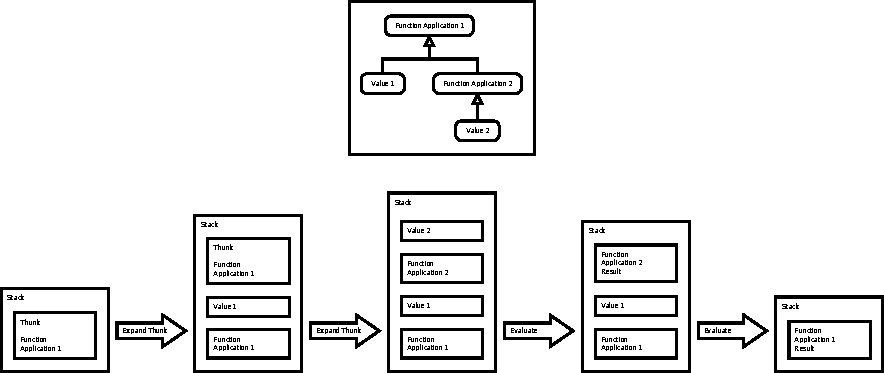
\includegraphics[width=\textheight]{../diags/eval-stack.pdf}

\caption{Overly simplified concept sketch of the evaluation stack; 
when the first Application is to be evaluated, it is discovered that it
contains unevaluated expressions. The Application is turned into a Thunk.
The Thunk is then popped from the stack, and the Application is added to
the stack, the Application arguments are popped on the stack with any 
Applications turned into thunks. The top of the stack is again a Thunk.
The same routine is performed on the new Thunk, until the expression top
Application can be reduced to a Value. After this, the initial Application
can also be reduced to a Value.
}
\label{fig:sketch}

\end{figure}
\end{sidewaysfigure}

\end{comment}

\subsection{Extensions}

This project involved extending Haskell-Python to a full Haskell interpreter 
through the use of GHC.

\subsubsection*{GHC usage}

% TODO

By using GHC to compile the Haskell programs and dump its intermediate
format to a file, we can effectively turn Haskell-Python into a full
Haskell compiler. However, the format dumped by GHC is External-Core.

We turn External-Core into JSCore with a Haskell program called "core2js".
JSCore is a JSON compliant representation of external-core. This means that
we can parse JSON and get a representation we can easily traverse when building
the AST (Abstract Syntax Tree) for the Core' interpreter.

\subsubsection*{Module system}

% TODO
A module system was implemented for the interpreter. A module object contains
a dictionary for variables, type-constructors and data-constructors. The 
"library" contains a dictionary of modules. This structure corresponds to the
module hierarchy used by GHC.

\subsubsection*{Parser}

% TODO

The parser is implemented using some of the PyPy parsing tools. A simple 
JSON grammar is described in EBNF form in a Python string. This string
is then parsed by the PyPy tool and a parser is created. By using this JSON
parser and traversing the resulting datastructure, we build the AST for the 
interpreter. See subsection \ref{chap:rewrite} for a detailed description of 
the parser and the Core to Core' mapping.

\subsubsection*{Primitives}

% TODO
The Primitive values extend the Value class. Primitive functions handle
these values.
See subsection \ref{chap:prims} for a more in-depth discussion of the
library and primitives.


%\clearpage


\chapter{From Core to Core'}


\section{The Case statement}


\section{Partial function application}


\section{Getting the primitive types}




%\clearpage


\chapter{System description}
\label{chap:impl}

This chapter discusses the implementation of the project with
references to the source tree (figure \ref{fig:overview}).
Note that the source tree has been refactored by E.W. Thomassen
to better fit with other PyPy projects. This subsection discusses how
and where the specific functionality is implemented. Note that there
are a number of problems with the current implementation, and that
these are discussed in chapter \ref{chap:conc}.

\section{Toplevel}

The toplevel of the source tree contains a "readme" file, a folder
called "pyhaskell" where the main interpreter functionality is 
implemented, and a file called "targethaskellstandalone.py" that 
defines the target and entry point for the PyPy translation tool.

\section{The main functionality}

The pyhaskel folder contains 3 main programs. "main.py",
"makegraph.py" and "run\_tests.py".

"main.py" is the entry point of the compilation system. It defines
the target for the RPython translation tool, imports the \emph{builtin}
functionality and the main function begins the interpretation of the
JSCore program.

The program "makegraph.py" contains a JSON parser and dumps the resulting
JSON tokens to a dot file in order to generate a graph using the graphviz
tool.

The "runtests.py" program contains a program that executes all the programs
in the sub folder "test" and then prints the result of the tests.

\begin{sidewaysfigure}
\begin{figure}[H]
\centering
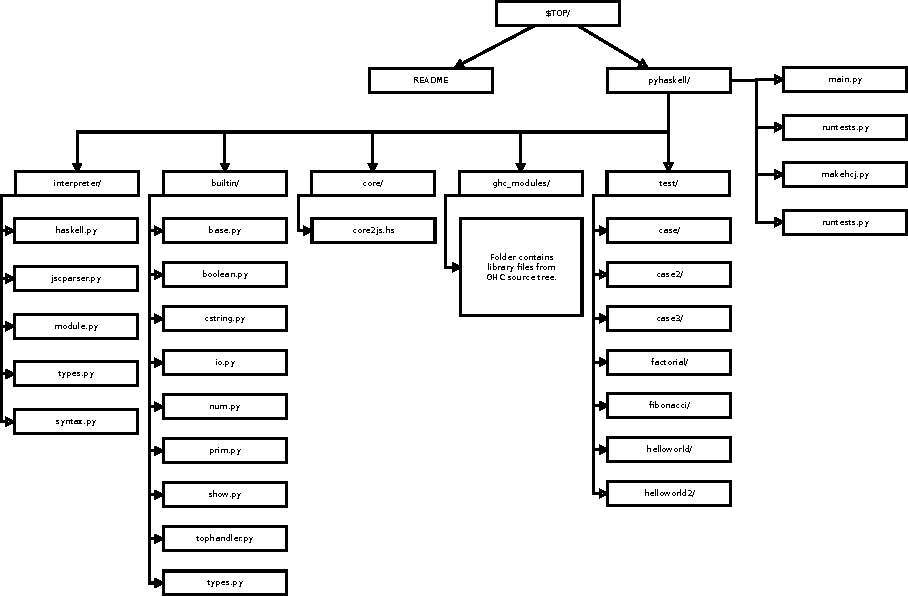
\includegraphics[width=\textheight]{../diags/overview.pdf}

\caption{Overview of source tree}
\label{fig:overview}

\end{figure}
\end{sidewaysfigure}

The sub folder "interpreter" contains the actual
interpreter code, the parser and the module system implementation. These are
discussed in the following sections.

\subsection*{Interpreter}

The file "haskell.py" in the folder "interpreter" contains the
Haskell-Python interpreter, the base of the compilation system.
This subsection describes the keys of the Haskell-Python implementation.
See figure \ref{fig:coreinterp} for a class diagram.

Haskell-Python consists of a few base classes; 

\begin{itemize}

\item \emph{Symbol} contains a static dictionary of all Symbols. This is 
simply used to compare "names" by their object identity.

\item \emph{HaskellObject} is a base class for all objects handled by the
interpreter.

\item \emph{Value} is a base class for evaluated values.

\item \emph{Constructor} inherits from \emph{Value} and implements an abstract 
base class for constructors with different number of arguments.

\item \emph{ConstructorN} inherits from \emph{Constructor} and is used as the 
base for a number of other Constructor classes created by a function called 
\emph{make\_arg\_subclass}. This function is again called by another function
called \emph{make\_constructor} that creates a Constructor based on the length
of the list it receives as argument. And this function (\emph{make\_constructor})
is called by another function \emph{constr} takes the name-argument (a string)
and looks it up in the list of symbols to create the actual Constructor. So the
actual Constructor is created by a coll to the function \emph{constr(name, *args)}.

\item \emph{AbstractFunction} inherits from \emph{Value} and is the base class for 
the functions of Haskell-Python. 

\item \emph{Function} inherits from AbstractFunction and defines a user-defined 
Haskell-Python function, it contains a name and a list of \emph{Rules}

\item \emph{Rule} is a field of the Function. It consists of a list of patterns and
an expression. If the function is applied and its arguments matches a pattern, the
expression is evaluated.

\item \emph{Substitution} inherits from HaskellObject and is the body of a function 
with its numbered variables substituted by values.

\item \emph{PrimFunction} inherits from \emph{AbstractFunction} and describes a function
implemented at the machine level. A function called \emph{expose\_primitive} is
can be used as a python-decorator to create \emph{PrimFunction} objects.

\item \emph{Var} inherits from \emph{HaskellObject} and describes a Haskell variable. 

\item \emph{NumberedVar} inherits from \emph{HaskellObject}. A \emph{Var} is replaced
by a \emph{NumberedVar} by a call object-function \emph{enumerate\_head} inherited from
\emph{HaskellObject} when creating a \emph{Rule}.

\item \emph{Application} inherits from \emph{HaskellObject} and describes an
abstract base class for Haskell-Python function application. Like the constructor,
classes are created by a function for various number of arguments.

\item \emph{ApplicationN} inherits from \emph{Application} and is used by the function
\emph{make\_application} to create Application classes with various number of arguments.
This function, like \emph{make\_constructor} is used by the function 
\emph{make\_arg\_subclasses} to create Applications with various number of arguments.

\item \emph{Thunk} inherits from \emph{HaskellObject} and represents an unevaluated
function application. 

\item \emph{StackElement} is a base class for the elements of the evaluation stack.

\item \emph{CopyStackElement} inherits from \emph{StackElement} and contains a
\emph{Application}.

\item \emph{UpdateStackElement} inherits from \emph{StackElement} and contains a
\emph{Thunk}. The \emph{Thunk} contained in the object is updated after its 
content has been evaluated.
\end{itemize}

In addition to these classes, the most important functions are;

\begin{itemize}

\item \emph{expose\_primitive} and the following two functions have already been 
mentioned. \emph{expose\_primitive} can be used as a python-decorator.

\item \emph{constr} creates a \emph{Constructor} object by looking up the "name" in
the dictionary of the \emph{Symbol} class, and selecting the correct sub-class from the
sub-classes generated for \emph{Constructor}.

\item \emph{make\_application} is similar to \emph{make\_constructor}, there is no
need for a wrapper function as it does not have to look up a \emph{Symbol}.

\item \emph{main\_loop} is the main function, it reduces a Haskell-Python 
\emph{Application} to a \emph{Value}. The function \emph{evaluate\_hnf} is
simply a wrapper for the \emph{main\_loop function}
\emph{main\_loop}.

\end{itemize}

This section has described the Haskell-Python implementation in detail, based
on the classes and functions implemented.

\begin{sidewaysfigure}
\begin{figure}[H]
\centering
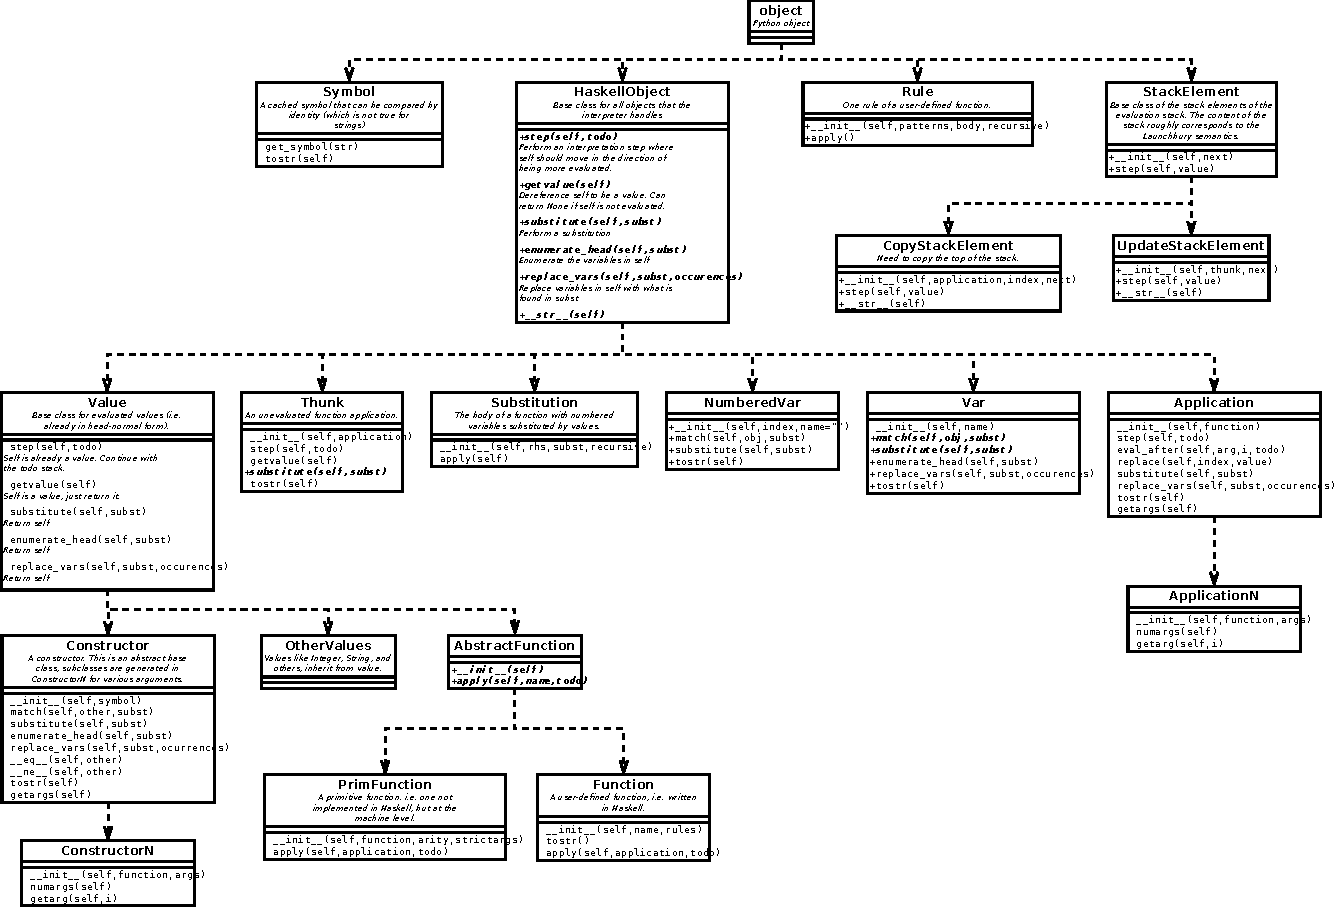
\includegraphics[width=\textheight]{../diags/core-interp.pdf}

\caption{Haskell-Python class diagram}
\label{fig:coreinterp}

\end{figure}
\end{sidewaysfigure}

\subsection*{Primitive types}

The file "primtypes.py" in the folder "interpreter" contains the primitive types
for the Haskell-Python interpreter. The types implemented inherit from the
\emph{Value} class in "haskell.py".

The following primitive types are implemented;

\begin{itemize}
\item \emph{Char} represents a single Haskell character-value.
\item \emph{Int} represents a Haskell Int value.
\item \emph{Addr} is a memory address. Among other it is used to represent
the String type.

\item \emph{Double} is simply a double precision floating point value.
\item \emph{Float} is simply a single precision floating point value
\end{itemize}

Since these classes all inherit from the Value type of Haskell-Python, 
they have a common interface; they all contain a variable called value that
contain its actual contents. This is currently implemented as a python
variable, so it is not represented like its Haskell equivalent at the low-level.
See listing \ref{lst:int1} for an example of how a primitive value is implemented.

\begin{figure}[H]
\lstset{ %
language=Python,
caption=Python class implementing the Haskell Int Value.,
label=lst:int1
}
\begin{lstlisting}
class Int(haskell.Value):
    _immutable_fields_ = ["value"]

    def __init__(self, integer):
        assert isinstance(integer, int)
        self.value = integer

    def match(self, other, subst):
        value = other.getvalue()
        if value:
            assert isinstance(value, Int)
            if self.value == value.value:
                return haskell.DEFINITE_MATCH
            return haskell.NO_MATCH
        return haskell.NEEDS_HNF

    def __eq__(self, other):
        return (isinstance(other, Int) and self.value == other.value)

    def __ne__(self, other):
        return not (self == other)

    def tostr(self):
        return str(self.value)
\end{lstlisting}
\end{figure}


\subsection*{Modules}

The file "module.py" in the folder "interpreter" contains the basics of the
module system. It contains a single class; \emph{CoreMod}. This class corresponds
to a Haskell Module. A \emph{CoreMod} object contains a name, and three dictionaries.
These dictionaries are called \emph{qvars}, \emph{qtycons} and \emph{qdcons} and they
contain \emph{qualified variables}, \emph{qualified type constructors} and 
\emph{qualified data constructors} respectively. When a \emph{CoreMod} object is created
it is at once added to the list of Haskell Modules.

\subsection*{JSCore parser}

The file "jscparser.py" in the "interpreter" folder contains the parser code. 
This code is responsible for loading JSCore files, and creating the AST based 
on the interpreter and module-system implementations.

The parser implementation takes advantage of some of the parsing tools 
available from
the PyPy code base. By writing an EBNF grammar for JSON, and giving it to a 
function called \emph{parse\_ebnf}, a JSON parser is created.

The resulting parser is a base class called \emph{RPythonVisitor}. The 
RPythonVisitor
class implements \emph{visit} functions for the constructs created by the 
EBNF grammar. For JSON this becomes \emph{visit\_object}, 
\emph{visit\_number} etc.

The result of this is that we have a set of functions that get called when 
visiting JSON constructs. Since JSCore is a description of External-Core 
compatible with JSON this lets us parse the Core programs by branching 
on the visitor functions.

This way, the mapping described in \ref{chap:rewrite} is implemented.

\section{Built-in functionality}

The "builtin" folder contains all the Haskell library functionality that
have been implemented in Python. Most of this functionality should have been
stored in the sub folder "ghc\_modules" as JSCore files. However, due to some 
issues that are discussed in conclusions and future work, this is not currently
the case.

As an example, the file "num.py" contains the implementation for the generic
Num class. Listing \ref{lst:zmnum} contains the implementation for the
generic minus function. Currently it only supports the Int type. Note that
it takes three arguments, the first argument is used to resolve which 
function actually implements the minus function, and the other two are the
arguments for this function.

\begin{figure}[H]
\lstset{ %
language=Python,
caption=Python class implementing the Haskell Int Value.,
label=lst:zmnum
}
\begin{lstlisting}
@haskell.expose_primitive(3)
def zm( args ):
    ty = args[0]
    a = args[1]
    b = args[2]

    if ty == mod.qvars["$fNumInt"]:
        return haskell.make_partial_app(izhconstr,
            [haskell.make_partial_app(prim.zmzh, [a.getarg(0), b.getarg(0)])])
    else:
        raise NotImplementedError

mod.qvars["-"] = zm
\end{lstlisting}
\end{figure}

\section{External-Core to JSCore}

The "core" folder contains the Haskell program responsible for generating the
JSCore intermediate format. This program is called "core2js". Currently, the
program uses the External-Core parser from the "extcore" Haskell package and
the JSON package to read the Haskell file in External-Core format and dump it
in JSCore format.

\section{GHC modules}

The folder "ghc\_modules" contain the GHC boot libraries. And a script that 
takes all these Haskell modules and uses GHC to create External-Core files
using the "-fext-core" flag and "core2js" to create JSCore files from the 
resulting External-Core files.

The GHC library files are organized exactly as in the GHC source tree. Each
folder in the "libraries" directory corresponds to a Haskell package. These
packages contain the Haskell modules. E.g. the module "GHC.Tuple" is located
in "ghc-prim/GHC/Tuple.hs".

\section{Tests}

The "test" directory contains one subdirectory for each test. The
subdirectories contain a single Haskell file with the same name as the
subdirectory (other files are created and put in the directory when running
the test). E.g. the test "fibonacci" is located in the following path:
"test/fibonacci/fibonacci.hs" and after running the test the "fibonacci"
folder should contain the additional files; "factorial.hcr", "factorial.hi",
"factorial.o" and "factorial.hcj". ".hcj" is the extension used for JSCore
files.

The output from running the test script is:

\begin{figure}[H]
\lstset{ %
language=Python,
caption=Output from running the test script,
label=lst:testoutput
}
\begin{lstlisting}
-----------------------
Results (29.96 seconds)
-----------------------
case :  Success
data :  Success
factorial :  Success
fibonacci :  Success
helloworld :  Success
let :  Success
multiply :  Success
partialapp :  Success
\end{lstlisting}
\end{figure}

\begin{comment}

\subsection{Pipeline}
\label{chap:pipe}

This subsection contains a description of the pipeline currently implemented.

\subsubsection*{Haskell to extcore}

When running a Haskell file using this system, the file is first processed
by GHC.

\subsubsection*{Extcore to JSCore}

\begin{itemize}
\item extcore
\item linkcore ?
\end{itemize}

\subsubsection*{JSCore to Core'}

\subsubsection*{Parsing and interpretation}





\subsection{Testing}
\label{chap:test}

\subsubsection*{Current testing of interpreter}

The current testing used on the project is done by a python-script that performs
the following actions:

\begin{itemize}

\item For all folders in folder 'test':

\begin{itemize}

\item Compile haskell program with GHC and dumping to external-core

\item Run the core2js program on resulting external-core file

\item Run the main interpreter on the JSCore file.

\end{itemize}

\item Dump return-values of programs.

\end{itemize}

Our testing should be extended by checking if the output is correct.


\subsubsection*{GHC test suit}

GHC uses a testsuit. Getting the interpreter to pass these tests are the
ultimate goal, however, the project is not there yet.

\end{comment}

%\clearpage
%

\chapter{Primitives and Libraries}
\label{chap:prims}



\section{The initial plan}

GHC uses a module called GHC.Prim, located in the ghc-prim package. This
module is generated automatically from a file called "primops.txt.pp", this file
contains information about the machine representations of the various types, as
well as the operations that can be performed on them.

Initially, it was assumed that it would be trivial to translate the Haskell
libraries used by GHC into External-Core using GHC. This way, it would only 
be necessary to implement the primitive types and functions.

The External-Core functionality of GHC has bitrotted, and because of this, it can't be
used to create External-Core files for all the GHC libraries. This is a GHC bug. 
Although it produces correct
External-Core for some Haskell code, it does not for all. Since many crucial library files
can not be created External-Core for, we can not continue to use this approach.

\section{Our approach}

Currently, GHC is used to parse, typecheck, desugar and generate the 
External-Core representation of our program. By implementing the
primitive types and library functionality in Python, we are able to
get some simple programs running.


\section{Why it does not work}

% TODO: Libraries use Haskell code not supported by the External-Core libraries.

The initial reasoning for using External-Core was as follows;
it has a clearly defined syntax that is easy to work with, and it was 
assumed that it was decently supported. Unfortunately, there are bugs in
the parts of GHC responsible for generating External-Core, this in turn
results in the fact that we are unable to create External-Core files for the
necessary libraries.


\section{How to fix it}

% TODO: Should i link to the bugs ???

GHC includes a library, it should be doable to use this library to get
GHCs own internal Core representation when compiling a file. Using this 
representation, it should be easy to create a JSCore-like format to use.

However, to do this, the step performing this must be a linked into the
actual GHC binary, as it is not possible to compile the Base package without
actually compiling GHC. This is also due to a bug in GHC.

\section{Our current implementation}


% TODO: Present all library functionaliyt implemented !

Following is a description of some of the most notable implemented library 
functions.

All the builtin functionality is located in the "toplevel/pyhaskell/builtin/"
folder. When describing the implementation of a Value or a Function, we note
the Python file and the Haskell module it refers to.

\subsection{Primitive Values}

A few primitive Value types has been implemented. The ones that are currently
tested are Char and Int. See listing \ref{lst:int} for an example of a 
Value implementation. 

% TODO: _immutable_fields_ = ["value"] hit to the translator

\begin{figure}[H]
\lstset{ %
language=Python,
caption=Python class implementing the Haskell Int Value.,
label=lst:int
}
\begin{lstlisting}
class Int(haskell.Value):
    _immutable_fields_ = ["value"]

    def __init__(self, integer):
        assert isinstance(integer, int)
        self.value = integer

    def match(self, other, subst):
        value = other.getvalue()
        if value:
            assert isinstance(value, Int)
            if self.value == value.value:
                return haskell.DEFINITE_MATCH
            return haskell.NO_MATCH
        return haskell.NEEDS_HNF

    def __eq__(self, other):
        return (isinstance(other, Int) and self.value == other.value)

    def __ne__(self, other):
        return not (self == other)

    def tostr(self):
        return str(self.value)
\end{lstlisting}
\end{figure}

\subsection{Lists}

The cons (or, ":") constructor. A constructor is created with the "haskell.constr()"
function.

A Python-decorator is used to turn a Python function into a Haskell primitive function.
The decorator "@mod.expose(name, arity)" implemented in the Module class, turns a Python 
function into a haskell function by creating a PrimFunction and adding it to the 
variable-dictionary of the "mod" module. See \ref{lst:cons} for an example.

\begin{figure}[H]
\lstset{ %
language=Python,
caption=Implementation of the Haskell ++ (concatenation) operator.,
label=lst:cons
}

\begin{lstlisting}
mod = module.CoreMod("base:GHC.Base")

@mod.expose("++", 2)
def concatenation(args):
    def conc(a, b):
        if len(a.getargs() ) > 1:
            return haskell.constr(":", a.getarg(0), conc(a.getarg(1), b) )
        else:
            return b

    a, b = args
    t = conc(a,b)

    return t 
\end{lstlisting}
\end{figure}


The end of a list refors to a "[]" constructor (haskell.constr("[]")).


\subsection{unpackCString}

The unpackCString function is implemented simply. \ref{lst:unpack}




\begin{figure}[H]
\lstset{ %
language=Python,
caption=Implementation of the unpackCString function.,
label=lst:unpack
}

\begin{lstlisting}
mod = module.CoreMod("ghc-prim:GHC.CString")

@mod.expose("unpackCString#", 1)
def unpackCString(args):
    a = args[0]
    b = str(a.value)
    t = types.zmzn 
    for i in range(len(b)-1, -1, -1):
        c = haskell.constr( "Czh", Char(b[i]) )
        t = haskell.constr( ":", c, t )
    return t 
\end{lstlisting}
\end{figure}




 

\subsection{putStrLn}


\begin{figure}[H]
\lstset{ %
language=Python,
caption=Implementation of the putStrLn function.,
label=lst:put
}

\begin{lstlisting}
mod = module.CoreMod("base:System.IO")

@mod.expose("putStrLn", 1)
def putStrLn(args):
    t = args[0]
    while len(t.getargs()) > 1:
        sys.stdout.write( t.getarg(0).getarg(0).value )
        t = t.getarg(1)
    sys.stdout.write("\n")
    return args[0]
\end{lstlisting}
\end{figure}




\subsection{TopHandler}

base:GHC.TopHandler ....

runMainIO ....

wrapper for:
main ....

\subsection{The Num class}

The Num class implements some generic functions. The ones implemented
in our Python library is multiplication, subtraction and addition. These
are pretty much implemented in the same way, so we only present the
multiplication function as an example here, see listing \ref{lst:mul}.
Note that the function takes 3 arguments, the first argument 
(in the fibonacci test case, \$fNumInt) is used to tell the
generic multiplication function which specific function to use.
See section \label{subsec:classes} for a description. In our 
implementation however, the first argument is just an Int that we 
check against.

\begin{figure}[H]
\lstset{ %
language=Python,
caption=Implementation of the generic multiplication function.,
label=lst:mul
}

\begin{lstlisting}
@mod.expose("*", 3)
def multiply(args):
    ty, a, b = args
    if ty == mod.qvars["$fNumInt"]:
        return haskell.make_application(izhconstr,
            [haskell.make_application(prim.multiply, [a.getarg(0), b.getarg(0)])])
    else:
        raise NotImplementedError
\end{lstlisting}
\end{figure}



%\clearpage
%
\section{Testing}
\label{chap:test}

\subsection{Current testing of interpreter}

The current testing used on the project is done by a python-script that performs
the following actions:

\begin{itemize}

\item For all folders in folder 'test':

\begin{itemize}

\item Compile haskell program with GHC and dumping to external-core

\item Run the core2js program on resulting external-core file

\item Run the main interpreter on the JSCore file.

\end{itemize}

\item Dump return-values of programs.

\end{itemize}

Our testing should be extended by checking if the output is correct.


\subsection{GHC test suit}

GHC uses a testsuit. Getting the interpreter to pass these tests are the
ultimate goal, however, the project is not there yet.

%\clearpage
\chapter{Similar work}
\label{chap:similar}

In addition to the Python implementation, PyPy implements a low-level 
hardware emulator (PyGirl), a PHP interpreter, and a Prolog interpreter. 
Various other experiments have also been created by the PyPy team. This
chapter is a brief discussion of these projects and experiments. 

Some work has also been done on the GHC side, among others; a LLVM
(Low Level Virtual Machine) back-end has been implemented.

% TODO !
\section{The GHC LLVM back-end}

The LLVM (Low Level Virtual Machine) is a framework for the optimization of 
programs from the compilation phase to runtime. The LLVM provides high-level information 
to the compilation system during compile-time, run-time and in idle time between
runs. By creating code generators for the virtual instruction set supported by
LLVM, implementers can take full advantage of its features.
\cite{lattner2004llvm}

GHC can generate LLVM code from Cmm (C minus minus; is a low-level imperative
language with an explicit stack). In some cases the 
LLVM back-end can produce significantly faster code than the traditional route. 
\cite{marlow2012glasgow, terei2010llvm}

\section{PyPy Prolog}

In addition to the implementation of Python, PyPy has also shown that its techniques
are applicable to other languages. The Prolog VM is an example of this. Implementations
of Prolog are usually written in low-level languages such as C, this usually results in
good performance, but means they are difficult to write and maintain. The PyPy Prolog 
interpreter clearly outperforms other Prolog interpreters written in other high-level
languages, and it also outperforms state-of-the-art Prolog VMs at specific benchmarks,
which shows that other Prolog implementations can benefit from the techniques used by
PyPy. \cite{bolz2010towards}

% TODO !
\section{HappyJIT}

PHP (Hypertext Preprocessor) is a language used to develop the server-side of 
websites. The users request for a website is received by the server, the PHP script
then executes the request, often involving querying a database and then generating 
the actual HTML for the user. Increasing the effectiveness of this process would
reduce the time it takes for a user to have a website request answered. 
The HappyJIT project implements a PHP interpreter in RPython, this interpreter is 
translated by the PyPy translator into a tracing-JIT. The approach shows that 
the techniques significantly improve the performance of several common use cases.
\cite{homescu2011happyjit}

% TODO 
\section{PyGirl}

As a case study, PyGirl implements an emulator for the Nintendo Game Boy. The project 
shows the feasibility of implementing a low-level VM for hardware in a high-level 
language to improve portability, and reduce complexity. The project shows that the
reduction in implementation complexity with this approach is substantial, 
and that the performance loss can be insignificant.
\cite{bruni2009pygirl}





\chapter{Preliminary benchmarks}

This chapter briefly discusses the benchmarking that was done.

\section{Specifications}

The benchmarking was done on the following setup;

\begin{table}[H]

\centering
\begin{tabular}{l|l}

\hline
\hline
Processor & Intel Core i7-640M (2x2.8GHz) \\
Memory    & 2x2GB DDR3-1333 \\
Chipset   & Intel PM55 \\
OS        & Arch Linux (3.3.7-1-ARCH) \\
\hline
\end{tabular}

\caption{Relevant system specifications}

\end{table}

\section{Test program}

\ref{lst:naivfib}

\lstset{ %
language=Python,
caption=Naive fibonacci implementation in Haskell,
label=lst:naivfib
}
\begin{lstlisting}
main = do 
    let n = 40
    putStrLn $ "Fib(" ++ (show n) 
               ++ ") = " ++ (show $ fib n)

fib :: Int -> Int
fib 0 = 0
fib 1 = 1
fib n = fib (n-1) + fib (n-2)
\end{lstlisting}

\section{Results}

The benchmarking was done by running the naive fibonacci program with $n=40$ 
on the Intel Core i7-640M processor. The results can be seen in table 
\ref{tab:benchmarks}. GHC version 7.4.1 was used. 

\begin{table}[H]

\centering
\begin{tabular}{l|l}
\hline
\hline
Compilation System & Time \\
\hline
GHC               & 0m 11.296s  \\
runhaskell        & 4m 23.803s \\ 
PyHaskell no JIT  & 12m 57.254s \\
PyHaskell JIT     & 1m 20.638s \\
\hline
\end{tabular}

\caption{Timing results for running the naive fibonacci implementation with n=40. Results
are from the "user" output of the "time" linux command.}
\label{tab:benchmarks}

\end{table}

From these results it is clear that the interpreter must be optimized further if
it is to compete with GHC. A significant decrease in execution time with the JIT
as opposed to without the JIT was observed. In addition, for this benchmark, the
interpreter with JIT was approximately $3.3$ times faster than $runhaskell$ 
(an interpreter that comes with GHC).






\chapter{Conclusion and Future Work}
\label{chap:conc}


\section{Serializing and deserializing}
\label{serdes}

The current situation regarding the serialization of Haskell programs into 
the JSCore format have several problems. It is dependent on a buggy part of GHC, 
and on a poorly maintained package (extcore). The result of these bugs is that
GHC exits with a panic-error when compiling some Haskell modules. And this in
turn, means that we have been unable to create JSCore for the GHC boot libraries.

Currently, the libraries necessary to run some simple Haskell programs have been
implemented at a high level in Python. This implementation is not "correctly"
implemented with regard to the Haskell language, but it is sufficient in order
to test some simple programs.

Some alternative methods have been investigated as solutions for this problem,
including the use of the Cabal (Haskell package system) API in collaboration
with the GHC API in order to create the JSCore files. However, Cabal interface
with GHC through command line arguments. 
It was also attempted to create the necessary functionality using just the GHC
API, however this also turned out to be problematic. Though it now seems like
this is the best way to move forward. By using the main module as the base for
the serializer, it should be possible to interface with the build-system
exactly like GHC does. This would mean that it would be possible to write a
fairly simple Haskell function to dump the intermediate format used by GHC
to JSCore, and since this program would function exactly like GHC, anything 
would be possible to compile using it.

The deserialization should not change much, as the JSCore intermediate format
would not have to change very much. If anything, the JSCore format can be
simplified, and made to match better against Core and System $F_C$ than
External-Core does. It is however, necessary to improve the serialization
functionality before the deserialization can be improved much as the programs
that can be serialized is of little complexity, and therefore does not test
very much.


\section{Benchmarking and testing}

Some simple benchmarking and testing was done. The benchmarking was done by
running the naive fibonacci program with $n=40$, the results can be seen in
table \ref{tab:benchmarks}.
It is clear that the interpreter must be optimized 
further if it is to compete with GHC. A significant increase in execution 
time with the JIT as opposed to without the JIT was observed. In addition,
for this benchmark, the interpreter with JIT was approximately $3.3$ times faster than
$runhaskell$ (an interpreter that comes with GHC).



The testing performed has been described in chapter \ref{chap:impl}. The results of the 
testing is that the current implementation is sufficient for simple programs taking 
advantage of various Haskell constructs. It is also clear that this is not sufficient
to run any more complicated programs, but it serves well for the future development of
the system. Eventually, the interpreter should run the GHC benchmarking suite (NoFib) and 
the GHC testsuit.

\section{Concluding remarks}

%NoFib GHC benchmark

The goals of this project was to investigate whether Haskell could benefit from JIT 
compilation, specifically; the techniques applied by the PyPy project. 
To answer this, it was attempted to implement a full Haskell compilation
system, using an interpreter called Haskell-Python\cite{haskellpython} as the back-end,
and GHC as the front-end, and translate it into a JIT compiler using the PyPy translation
toolchain. The work involved in this project has mostly been the implementation of the necessary
tools to get Haskell programs from GHC into Haskell-Python. This has only been partially
successful, as discussed in section \ref{serdes}.

Unfortunately, the original question remains unanswered at this stage, as the
approach taken to test the hypothesis has not been successfully completed. However,
based on the results from this partially implemented system, its continued
development may result in a fast Haskell compilation system, and may eventually prove
the hypothesis true.



%\clearpage
%\section{Future work}

\subsection{Getting programs into Haskell-Python from GHC}

This project focused mainly on this task, which was thought to be simple.
However, due to a combination of reasons, this turned out not to be the case.
Mainly, inexperience; with Haskell, the GHC API, and functional languages in 
general. However, a lot of experience was gained during this project, and
future development will benefit from this.

The work involved in this will be revisiting the different possibilities to
achieve our goal. Some options are:

\begin{itemize}
\item Write an external-core parser directly in RPython, and use files generated by GHC.
\item Include development of extcore as a part of the project. This is most likely a bad
idea, as this seems to be no easier than the alternatives.
\item Use the GHC API to generate JSCore, this is also nontrivial.
\item Create functionality to be linked into the GHC executable, in order to generate the
representation of JSCore. Also nontrivial.
\item Simply use the version of GHC matching the version of extcore. This will not be
a good idea for further development of the project, but may be a simple solution to get
a prototype working quickly.
\item Implement a Haskell pipeline in RPython, including parsing, typechecking and desugaring.
This will be a very large task.
\end{itemize}

Either way, understanding of Haskell and Core must be a top priority.

\subsection{Rewrite the deserializer to proper RPython}

The deserializer is currently not written in proper RPython. 
Converting the code to RPython will allow it to be compiled to a JIT interpreter by
the RPython toolchain. This should not be a very big task, but it requires understanding
of the RPython coding style. There are also restrictions on how one may use the PyPy parser
tools.

\subsection{Implement basic Haskell libraries}

Implementing Haskell libraries is necessary to run any Haskell program passed 
through GHC. One option may be to implement (or automatically generate from GHC code) Haskell
primitive types, and to convert the Haskell base libraries to JSCore (or any other format that
may be chosen).

\subsection{Linking functionality}

Currently no thought has been given to the linking between multiple modules. This
must be implemented for any non-trivial Haskell programs to function.

\subsection{Test suite and benchmarking}

A framework for testing and benchmarking should be set up. Allowing us to compare
speed to other implementations, and progress of development. GHC uses a test framework
relying on Python and GNU Make that should be looked into.

\begin{comment}
\subsection{Map GHC encoded Types to Haskell-Python}

Figure out how to create encoded types for Haskell-Python. It may be possible to
autogenerate these from GHC files.

"2.) understanding how GHC encodes types. The Core Haskell of the previous steps encodes the types of all functions in slightly low-level
ways. This needs to be understood and a mapping of these types to what
the Python Haskell interpreter provides needs to be written." 

\subsection{Set up GHC test environment for Haskell-Python}

Setting up the GHC test environment for Haskell-Python would be very valuable
for development and bug fixing.

"3.) the actual interpretation of the Core language is mostly
implemented. There are probably some things missing, which will be
discovered by running some Haskell programs. For that end, it would be
good to find out whether there is a Haskell implementation test suite
and get it to run."

\subsection{Add built in Haskell types to run some Haskell benchmarks}

"4.) what is missing to run more non-pure Haskell programs are all the
built-in functions (e.g. those that perform arithmetic, I/O, call C
functions, etc) and built-in types (e.g. integers, floats, C-level types
like arrays and structs). These should be added step by step. This is an
essentially open-ended task. It would be good to add as many built-ins
so that some of the Haskell benchmarks can run."

\subsection{Optimize PyPy JIT for Haskell-Python}

"5.) JIT work: While the JIT of PyPy can mostly be automatically applied,
in practice a lot of careful work is needed to make sure that the
generated code is optimal (or at least good). To do that, a test suite
of Haskell snippets that explicitly compares the generated machine code
with what it should look like is needed, and then the careful adding of
some tests to this suite, together with the better placement of JIT
hints. This is both the hardest step, as well as the most exciting one."
\end{comment}


\clearpage
\bibliographystyle{plain}
\bibliography{papers}

\clearpage
\appendix
\appendixpage

\section{Formal definition of External-Core}
\label{coregrammar}


The following semantics is used to define the Core grammar, 
as seen in \cite{tolmach2010ghc}:

\begin{scriptsize}

\begin{longtable}{ l c l }

$[$ pat $]$		& :	& optional			\\
$\{$ pat $\}$		& :	& zero or more repetitions	\\
$\{$ pat $\}^{+}$	& :	& one or more repetitions	\\
$pat_{1}|pat_{2}$	& :	& choice			\\

\end{longtable}




\begin{grammar}
<module> ::= \%module <mident> \{ <tdefg> ; \} \{ <vdefg> ; \}
\end{grammar}

\paragraph{Type definitions}

\begin{grammar}
<tdefg> ::= \%data <qtycon> <tbind> = <cdef>
       \alt \%newtype <qtycon> <qtycon> <tbind> = <ty>
\end{grammar}

\paragraph{Constructor definitions}

\begin{grammar}
<cdef> ::= <qdcon> \{ @ <tbind> \} \{ <aty> \}
\end{grammar}

\paragraph{Value definitions}

\begin{grammar}
<vdefg> ::= \%rec \{ <vdef> \{ ; <vdef> \} \}
       \alt <vdef>
\end{grammar}

\begin{grammar}
<vdef> ::= <qvar> :: <ty> = <exp>
\end{grammar}

\paragraph{Atomic Expressions}

\begin{grammar}
<aexp> ::= <qvar>
      \alt <qdcon>
      \alt <lit>
      \alt ( <exp> )
\end{grammar}

\paragraph{Expression}

\begin{grammar}
<exp> ::= <aexp>
     \alt <aexp> \{ <arg> \}
     \alt \textbackslash \{ <binder> \} -$>$ <exp>
     \alt \%let <vdefg> \%in <exp>
     \alt \%case (<aty>) <exp> \%of <vbind> \{<alt> \{ ; <alt> \}  \}
     \alt \%cast <exp> <aty>
     \alt \%note " \{ <char> \} " <exp>
     \alt \%external ccall " \{ <char> " \} <aty>
     \alt \%dynexternal ccall <aty>
     \alt \%label " \{ <char> \} "
\end{grammar}

\paragraph{Argument}

\begin{grammar}
<arg> ::= @ <aty>
     \alt <aexp>
\end{grammar}

\paragraph{Case alternative}

\begin{grammar}
<alt> ::= <qdcon> \{ @ <tbind> \} \{ <vbind> \} -$>$ <exp>
     \alt <lit> -$>$ <exp>
     \alt \%\_ -$>$ <exp>
\end{grammar}

\paragraph{Binder}

\begin{grammar}
<binder> ::= @ <tbind>
        \alt <vbind>
\end{grammar}

\paragraph{Literal}

\begin{grammar}
<lit> ::= ( [-] \{ <digit> \} :: <ty> )
     \alt ( [-] \{ <digit> \} \% \{ <digit> \} :: <ty> )
     \alt ( <char> :: <ty> )
     \alt ( \{ <char> \} )
\end{grammar}

\paragraph{Value binder}

\begin{grammar}
<vbind> ::= ( <var> :: <ty> )
\end{grammar}

\paragraph{Type binder}

\begin{grammar}
<tbind> ::= <tyvar>
       \alt ( tyvar :: <kind> )
\end{grammar}

\paragraph{Atomic type}

\begin{grammar}
<aty> ::= <tyvar>
     \alt <qtycon>
     \alt ( <ty> )
\end{grammar}

\paragraph{Basic type}

\begin{grammar}
<bty> ::= <aty>
     \alt <bty> <aty>
     \alt \%trans <aty> <aty>
     \alt \%sym <aty>
     \alt \%unsafe <aty> <aty>
     \alt \%left <aty>
     \alt \%right <aty>
     \alt \%inst <aty> <aty>
\end{grammar}

\paragraph{Type}

\begin{grammar}
<ty> ::= <bty>
    \alt \%forall \{ <tbind> \} . <ty>
    \alt <bty> -$>$ <ty>
\end{grammar}

\paragraph{Atomic kind}

\begin{grammar}
<akind> ::= *
       \alt \#
       \alt ?
       \alt <bty> :=: <bty>
       \alt ( <kind> )
\end{grammar}

\paragraph{Kind}

\begin{grammar}
<kind> ::= <akind>
      \alt <akind> -$>$ <kind>
\end{grammar}


\paragraph{Names}

\begin{grammar}
<mident>	  ::= 	 '' <pname> : <uname> ''
	
<tycon>		  ::= 	 '' <uname> ''
		
<qtycon>	  ::= 	 '' <mident> . <tycon> ''

<tyvar>		  ::= 	 '' <lname> ''
	
<dcon>		  ::= 	 '' <uname> ''
	
<qdcon>		  ::= 	 '' <mident> . <dcon> ''

<var>		  ::= 	 '' <lname> ''

<qvar>		  ::= 	 '' || <mident> . || <var> ''

<lname>		  ::= 	 <lower> \{ <namechar> \}
 
<uname>		  ::= 	 <upper> \{ <namechar> \}

<pname>		  ::= 	 \{ <namechar> \}$^+$

<namechar>	  ::= 	 <lower> | <upper> | <digit>

<lower>		  ::= 	 a|b|...|z|\_

<upper>		  ::= 	 A|B|...|Z|

<digit>		  ::= 	 0|1|...|9									 


\end{grammar}




\end{scriptsize}


\chapter{Formal definition of JSCore}
\label{jscoregrammar}


\begin{grammar}
<module> 	::= \{ ''\%module'' : <mident> , ''tdefg'' : [ <tdefg> ] , ''vdefg'' : [ <vdefg> ] \}
\end{grammar}

\paragraph{Type definitions}

\begin{grammar}
<tdefg> 	  ::= 	 \{ ''\%data'' : <qtycon> , ''tbind'' : [ <tbind> ], ''cdef'' : [ <cdef> ] \}						
		  \alt 	 \{ ''\%newtype'' : <qtycon> , ''qtycon'' : <qtycon> , ''tbind'' : [ <tbind> ] , ''ty'' : <ty> \} 	

\end{grammar}

\paragraph{Constructor definitions}

\begin{grammar}


<cdef>		  ::= 	 \{ ''qdcon'' : <qdcon> , ''tbind'' : [ <tbind>  ] , ''aty'' : [<aty>]$^{+}$ \} 				 			

\end{grammar}

\paragraph{Value definitions}

\begin{grammar}

<vdefg>		  ::= 	\{ ''\%rec'' : [ <vdef> ]$^{+}$ \}    							
		  \alt 	<vdef>
<vdef> 		  ::= 	\{ ''qvar'' : <qvar> , ''ty'' : <ty> , ''exp'' : <exp> \}

\end{grammar}

\paragraph{Atomic Expressions}
\begin{grammar}


<aexp>		  ::= 	 \{ ''qvar'' : <qvar> \}
		  \alt 	 \{ ''qdcon'' : <qdcon> \}
		  \alt 	 \{ ''lit'' : <lit> \}
		  \alt 	 \{ ''exp'' : <exp> \} 


\end{grammar}

\paragraph{Expressions}

\begin{grammar}

<exp>		  ::= 	 <aexp>
		  \alt 	 \{ ''aexp'' : <aexp> , ''args'' : [ <arg> ]$^{+}$ \} 				
		  \alt 	 \{ ''lambda'' : [ <binder> ] , ''exp'' : <exp> \}		
		  \alt 	 \{ ''\%let'' : <vdefg> , ''\%in'' : <exp> \}				
		  \alt 	 \{ ''\%case'' : <aty> , ''exp'' : <exp> , ''\%of'' : <vbind>, ''alt'' : [ <alt> ]$^{+}$ \}	
		  \alt 	 \{ ''\%cast'' : <exp> , ''aty'' : <aty>	\}		
		  \alt 	 \{ ''\%note'' : ''  \{ <char> \} '' , ''exp'' : <exp>	\}	
		  \alt 	 \{ ''\%external ccal'' : '' \{ <char> \} '' , ''aty'' : <aty> \}	
		  \alt 	 \{ ''\%dynexternal ccal'' : <aty> \}
		  \alt 	 \{ ''\%label'' : '' \{ <char> \} '' \}


\end{grammar}

\paragraph{Argument}

\begin{grammar}

<arg>		  ::= 	 \{ ''aty'' : <aty> \}											 
		  \alt 	 \{ ''aexp'' : <aexp> \}										


\end{grammar}

\paragraph{Case alternative}
\begin{grammar}

<alt>		  ::= 	 \{ ''qdcon'' : <qdcon> , ''tbind'' : [ <tbind> ] , ''vbind'' : [ <vbind> ] , ''exp'' : <exp> \}
		  \alt 			 \{ ''lit'' : <lit> , ''exp'' : <exp> \}
		  \alt 			 \{ ''\%\_'' : <exp> \}	


\end{grammar}

\paragraph{Binder}

\begin{grammar}

<binder>	  ::= 	\{ ''tbind'' : <tbind> \}		
		  \alt 	\{ ''vbind'' : <vbind> \}	


\end{grammar}

\paragraph{Type binder}

\begin{grammar}

<tbind>		  ::= 	 \{ ''tyvar'' : <tyvar> \}
		  \alt 	 \{ ''tyvar'' : <tyvar> , ''kind'' : <kind> \}	


\end{grammar}

\paragraph{Value binder}

\begin{grammar}

<vbind>		  ::= 	 \{ ''var'' : <var> , ''ty'' <ty> \} 										 

\end{grammar}

\paragraph{Literal}

\begin{grammar}


<lit>		  ::= 	<jsstring>		 
		  \alt 	<jsnumber>


<jsstring>	  ::= 	 ''''														 
		  \alt 	'' <jschars> ''		
											 
<jschars>	  ::= 	<jschar>
		  \alt 	<jschar> <jschars>
												 
<jschar>	  ::= 	 See definition below

<jsnumber>	  ::=  	<jsint>
		  \alt 	<jsint> <jsfrac>
		  \alt 	<jsint> <jsexp>
		  \alt 	<jsint> <jsfrac> <jsexp>
											 
<jsint>		  ::= 	<jsdigit>
		  \alt  <jsdigit1-9> <jsdigits> 
		  \alt  - <jsdigit>
		  \alt  - <jsdigit1-9> <jsdigits>

<jsfrac> 	  ::=  	. <jsdigits>

<jsexp>		  ::=  	<jse> <jsdigits>

<jsdigits>	  ::=  	<jsdigit> 
		  \alt  <jsdigit> <jsdigits>

<jse>		  ::=  	e
		  \alt  e+		 
		  \alt  e- 		 
		  \alt  E		 
		  \alt  E+		 
		  \alt  E-

\end{grammar}

\paragraph{Atomic Type}

\begin{grammar}
<aty>		  ::= 	 \{ ''tyvar'' : <tyvar> \}
		  \alt 	 \{ ''qtycon'' : <qtycon> \}
		  \alt   \{ ''ty'' : <ty> \}

\end{grammar}

\paragraph{Basic Type}

\begin{grammar}
<bty>		  ::= 	 <aty>
		  \alt 	 \{ ''bty'' : <bty> , ''aty'' , <aty> \}
		  \alt 	 \{ ''\%trans'' : <aty> , ''aty'' : <aty> \}
		  \alt 	 \{ ''\%sym'' : <aty> \}
		  \alt 	 \{ ''\%unsafe'' : <aty> , ''aty'' : <aty> \}	
		  \alt 	 \{ ''\%left'' : <aty> \}
		  \alt 	 \{ ''\%right'' : <aty> \}	
		  \alt 	 \{ ''\%inst'' : <aty> , ''aty'' : <aty> \}


\end{grammar}

\paragraph{Type}

\begin{grammar}

<ty>		  ::= 	 <bty>
		  \alt 	 \{ ''\%forall'' :  [ <tbind> ]$^+$ , ''ty'' : <ty> \}	
		  \alt 	 \{ ''bty'' <bty> , ''ty'' : <ty> \} 


\end{grammar}

\paragraph{Atomic Kind}

\begin{grammar}

<akind>		  ::= 	 *	
		  \alt 	 \#
		  \alt 	 ?	
		  \alt 	 \{ ''bty'' : <bty< , ''bty'' : <bty> \}
		  \alt 	 \{ ''kind'' : <kind> \}	


\end{grammar}

\paragraph{Kind}

\begin{grammar}

<kind>		  ::= 	\{ ''akind'' : <akind> \}					
		  \alt 	\{ ''akind'' : <akind> , ''kind'' : <kind> \}		

<mident>	  ::= 	 '' <pname> : <uname> ''
	
<tycon>		  ::= 	 '' <uname> ''
		
<qtycon>	  ::= 	 '' <mident> . <tycon> ''

<tyvar>		  ::= 	 '' <lname> ''
	
<dcon>		  ::= 	 '' <uname> ''
	
<qdcon>		  ::= 	 '' <mident> . <dcon> ''

<var>		  ::= 	 '' <lname> ''

<qvar>		  ::= 	 '' || <mident> . || <var> ''

<lname>		  ::= 	 <lower> \{ <namechar> \}
 
<uname>		  ::= 	 <upper> \{ <namechar> \}

<pname>		  ::= 	 \{ <namechar> \}$^+$

<namechar>	  ::= 	 <lower> | <upper> | <digit>

<lower>		  ::= 	 a|b|...|z|\_

<upper>		  ::= 	 A|B|...|Z|

<digit>		  ::= 	 0|1|...|9									 


\end{grammar}



\section{Formal definition of JSON}
\label{jsongrammar}

\begin{scriptsize}
\begin{longtable}{ r c l r }
\multicolumn{4}{l}{Object}		\\
\\[0.01in]
$object$	& $ \rightarrow $ 	& \{ \}					& \\
 		& $ | $			& \{ $members$ \} 			& \\
$members$ 	& $ \rightarrow $	& $pair$				& \\
		& $ | $			& $pair$ , $members$ 			& \\
$pair$		& $ \rightarrow $	& $string$ : $value$ 			& \\
\\[0.01in]

\multicolumn{4}{l}{Array}		\\
$array$		& $ \rightarrow $	& [ ]					& \\
		& $ | $			& [ $elements$ ]			& \\
$elements$ 	& $ \rightarrow $	& $value$				& \\
		& $ | $			& $value$ , $elements$			& \\
\\[0.01in]

\multicolumn{4}{l}{Value}		\\
$value$		& $ \rightarrow $	& $string$				& \\
		& $ | $			& $number$				& \\
		& $ | $			& $object$				& \\
		& $ | $			& $array$				& \\
		& $ | $			& true					& \\
		& $ | $			& false					& \\
		& $ | $			& null					& \\
\\[0.01in]

\multicolumn{4}{l}{String}		\\
$string$	& $ \rightarrow $	& ""					& \\
		& $ | $			& " $chars$ "				& \\
$chars$		& $ \rightarrow $	& $char$				& \\
		& $ | $			& $char$ $chars$			& \\
$char$		& $ \rightarrow $	& any Unicode character except $"$ 	& \\ 
		&			& or $\backslash$ or control characters: & \\
		&			& $\backslash\backslash$		& \\
		&			& $\backslash /$ 			& \\
		&			& $\backslash b$ 			& \\
		& 			& $\backslash f$ 			& \\
		&			& $\backslash n$			& \\
		& 			& $\backslash r$ 			& \\
		&			& $\backslash t$ 			& \\
		& 			& $\backslash u$ four-hex digits\\
\\[0.01in]

\multicolumn{4}{l}{Number}		\\
$number$	& $ \rightarrow $ 	& $int$ 				& \\
		& $ | $			& $int$ $frac$				& \\
		& $ | $			& $int$ $exp$				& \\
		& $ | $			& $int$ $frac$ $exp$			& \\
$int$		& $ \rightarrow$ 	& $digit$				& \\
		& $ | $ 		& $digit1-9$ $digits$			& \\
		& $ | $ 		& - $digit$				& \\
		& $ | $ 		& - $digit1-9$ $digits$			& \\
$frac$ 		& $ \rightarrow $ 	& . $digits$ 				& \\
$exp$		& $ \rightarrow $ 	& $e$ $digits$ 				& \\
$digits$	& $ \rightarrow $ 	& $digit$				& \\
		& $ | $ 		& $digit$ $digits$			& \\
$e$		& $ \rightarrow $ 	& e					& \\
		& $ | $ 		& e+					& \\
		& $ | $ 		& e- 					& \\
		& $ | $ 		& E					& \\
		& $ | $ 		& E+					& \\
		& $ | $ 		& E-					& \\
\\[0.01in]

\caption{Grammar for JSON}
\label{json}
\end{longtable}

\end{scriptsize}




\end{document}
